\documentclass[pdftex,francais]{beamer}

% Copyright 2004 by Till Tantau <tantau@users.sourceforge.net>.
%
% This file can be redistributed and/or modified under
% the terms of the GNU Public License, version 2.

%% \ifx\themename\undefined
%%   \def\themename{default}
%% \fi

\usetheme{lama}
%\usetheme{Madrid}
%\usecolortheme{crane}

\usepackage{multirow}
\usepackage[latin1]{inputenc}           %%%  
\usepackage[T1]{fontenc}                %%%
\usepackage[francais]{babel}            %%%

\usepackage{multimedia}
\usepackage{hyperref}
\usepackage{tikz}
\usepackage{listings}

%\newtheorem{theorem}{Théorème}

%\setbeamercovered{transparent}

\title[Digital surfaces in DGtal]{Digital surfaces in DGtal\\
     Topology module (since 0.5)
}

\author[J.-O. Lachaud]{Jacques-Olivier Lachaud}

\date{DGtal Meeting, june 2012}


\graphicspath{{Figures/},{Images/},{Graphs/}}

%%% \AtBeginSection[]
%%% {
%%%   \begin{frame}<beamer>
%%%     \frametitle{Plan}
%%%     \tableofcontents[currentsection] %,currentsubsection]
%%%   \end{frame}
%%% }


\renewcommand{\vec}[1]{\mathbf{#1}}

% space of the real numbers
\newcommand{\R}{\ensuremath{\mathbb{R}}}
% space of the integer numbers
\newcommand{\Z}{\ensuremath{\mathbb{Z}}}
% Digitization process of step h (1)
\newcommand{\Dig}[1]{\ensuremath{\mathrm{Dig}_{#1}}}
% Family of shape
\newcommand{\SF}[0]{\ensuremath{\mathbb{F}}}
% Topological boundary of X (1).
\newcommand{\TB}[1]{\ensuremath{\partial #1}}
% Discrete geometric estimator of G (1)
\newcommand{\DGE}[1]{\ensuremath{E_{#1}}}
% Reference shape of digital object O (1) with grid step $h$ (2).
\newcommand{\RS}[2]{\ensuremath{R_{#1,#2}}}

% Digital contour.
\newcommand{\DC}{\ensuremath{C}}
% Continuous contour.
\newcommand{\CC}{\ensuremath{\mathcal{C}}}
% A point indexed by i (1) on the digital contour.
\newcommand{\PT}[1]{\ensuremath{\DC_{#1}}}
% A sequence of points indexed by i (1) on the digital contour.
\newcommand{\PTS}[2]{\ensuremath{\DC_{#1,#2}}}
% Predicate stating that the digital curve is a segment between indices 1 and 2
\newcommand{\SPRED}[2]{\ensuremath{S(#1,#2)}}
% ET logique
\newcommand{\AND}[0]{\ensuremath{\wedge}}
% OU logique
\newcommand{\OR}[0]{\ensuremath{\vee}}

% Tangent direction mapping of curve C (1)
\newcommand{\TGT}[1]{\ensuremath{\theta_{#1}}}
% Integral of squared curvature of curve C (1)
\newcommand{\ISC}[1]{\ensuremath{J[#1]}}
% Smallest possible tangent direction at constraint l (1)
\newcommand{\MinTD}[1]{\ensuremath{a_{#1}}}
% Largest possible tangent direction at constraint l (1)
\newcommand{\MaxTD}[1]{\ensuremath{b_{#1}}}
% Unknown tangent direction at constraint l (1)
\newcommand{\UnkTD}[1]{\ensuremath{t_{#1}}}

% ideal multiscale criterion
\newcommand{\IMSC}[2]{\ensuremath{\mu_{#1}(#2)}}
% multiscale profile
\newcommand{\MSP}[2]{\ensuremath{\mathcal{P}_{#1}(#2)}}
% threshold flat/curve
\newcommand{\CThreshold}[0]{\ensuremath{t_{f/c}}}
% threshold noise
\newcommand{\NThreshold}[0]{\ensuremath{t_{m}}}
% noise level
\newcommand{\NL}[0]{\ensuremath{\nu}}
% slope linear regression 
\newcommand{\SLR}[2]{\ensuremath{\theta_{#1}}}





% Pencil of maximal segments around a point.
\newcommand{\PE}[1]{\ensuremath{{\mathcal P}(#1)}}
% Tangent orientation of the maximal segment.
\newcommand{\TO}[1]{\ensuremath{\theta_#1}}
% lambda function for interpolation.
\newcommand{\LF}{\ensuremath{\lambda}}
% \lambda-MS tangent orientation.
\newcommand{\LTO}[1]{\ensuremath{\hat{\theta}(#1)}}
% \lambda-MS tangent orientation variation.
\newcommand{\LTOP}[1]{\ensuremath{\hat{\theta}'(#1)}}

%\definecolor{rougeSW_}{rgb}{0.968627,0.011765,0.015686}
\definecolor{darkgreen}{rgb}{0.0,0.6,0.0}
\definecolor{lightblue}{rgb}{0.5,0.5,1.0}
\definecolor{magenta}{rgb}{1.0,0.0,1.0}
\newcommand{\alertred}[1]{{\color{red}#1}}
\newcommand{\Cb}[1]{{\color{blue}#1}}
\newcommand{\Cdg}[1]{{\color{darkgreen}#1}}
\newcommand{\textmagenta}[1]{{\color{magenta}#1}}
\newcommand{\Implies}{{\ensuremath{\Rightarrow}}}

\newcommand{\Refs}[1]{{\color{lightblue}#1}}
\newcommand{\Cite}[1]{\Refs{[#1]}}
\newcommand{\Etal}{{\em et al.}}
\newtheorem{remark}{Remarque}
% Digitization process of step h (1)
\newcommand{\DigGh}[2]{\ensuremath{\mathrm{Dig}_{#2}(#1)}}
\newcommand{\BigT}{\ensuremath{\Theta}}
\newcommand{\BigO}{\ensuremath{O}}

\newcommand{\TAN}[0]{\ensuremath{\theta}}
% Position estimator
\newcommand{\EPOS}[0]{\ensuremath{\hat{{x}}}}
% Convexity Position estimator 
\newcommand{\ECONVPOS}[0]{\ensuremath{\hat{x}^\mathrm{conv}}}
% tangent estimator base MS.
\newcommand{\ETANMS}[0]{\ensuremath{\hat{\TAN}^{\text{MS}}}}
% tangent estimator base arete du CDP.
\newcommand{\ETANEDGE}[0]{\ensuremath{\hat{\TAN}^{\text{conv}}}}
% estimateur de longueur elementaire d'un surfel (1) sur le bord discretise de X(2) de pas h(3).

\newcommand{\Class}[1]{\alert{\texttt{#1}}}
\newcommand{\Concept}[1]{\texttt{\color{magenta}#1}}
\newcommand{\Method}[1]{\texttt{\color{lightblue}#1}}


\definecolor{MyGreen}{rgb}{0,0.6,0}

\setbeamercolor{qcolorb}{fg={blue!20!black},bg={blue!15!white}}
\setbeamercolor{qcolorub}{fg={blue!10!black},bg={blue!30!white}}
\setbeamercolor{qcolorlb}{fg={blue!20!black},bg={blue!8!white}}
\setbeamercolor{qcolorulb}{fg={blue!10!black},bg={blue!40!white}}
\setbeamercolor{qcolorg}{fg={green!20!black},bg={green!15!white}}
\setbeamercolor{qcolorug}{fg={green!10!black},bg={green!30!white}}
\setbeamercolor{qcolorlg}{fg={green!20!black},bg={green!8!white}}
\setbeamercolor{qcolorulg}{fg={green!10!black},bg={green!40!white}}
\setbeamercolor{qcolorr}{fg={red!20!black},bg={red!15!white}}
\setbeamercolor{qcolorur}{fg={red!10!black},bg={red!30!white}}
\setbeamercolor{qcolorlr}{fg={red!20!black},bg={red!8!white}}
\setbeamercolor{qcolorulr}{fg={red!10!black},bg={red!40!white}}
\newenvironment{myblockbluish}[2]%
	       {\begin{beamerboxesrounded}[lower=qcolorb,upper=qcolorub,width=#1,shadow=true]{#2}}{\end{beamerboxesrounded}}
\newenvironment{myblocklbluish}[2]%
	       {\begin{beamerboxesrounded}[lower=qcolorlb,upper=qcolorulb,width=#1,shadow=true]{#2}}{\end{beamerboxesrounded}}
\newenvironment{myblockgreenish}[2]%
	       {\begin{beamerboxesrounded}[lower=qcolorg,upper=qcolorug,width=#1,shadow=true]{#2}}{\end{beamerboxesrounded}}
\newenvironment{myblocklgreenish}[2]%
	       {\begin{beamerboxesrounded}[lower=qcolorlg,upper=qcolorulg,width=#1,shadow=true]{#2}}{\end{beamerboxesrounded}}
\newenvironment{myblockredish}[2]%
	       {\begin{beamerboxesrounded}[lower=qcolorr,upper=qcolorur,width=#1
,shadow=true]{#2}}{\end{beamerboxesrounded}}
\newenvironment{myblocklredish}[2]%
	       {\begin{beamerboxesrounded}[lower=qcolorlr,upper=qcolorulr,width=#1,shadow=true]{#2}}{\end{beamerboxesrounded}}

%%%%%%%%%%%%%%%%%%%%%%%%%%%%%%%%%%%%%%%%%%%%%%%%%%%%%%%%%%%%%%%%%%%%%%%%%%%%%%%
%%%%%%%%%%%%%%%%%%%%%%%%%%%%%%%%%%%%%%%%%%%%%%%%%%%%%%%%%%%%%%%%%%%%%%%%%%%%%%%
%%%%%%%%%%%%%%%%%%%%%%%%%%%%%%%%%%%%%%%%%%%%%%%%%%%%%%%%%%%%%%%%%%%%%%%%%%%%%%%
  \lstset{language=c++, numbers=left, tabsize=2, frame=single, breaklines=true, basicstyle=\ttfamily\scriptsize,
     numberstyle=\tiny\ttfamily, framexleftmargin=13mm, xleftmargin=12mm,keywordstyle=\color{blue}\bfseries,%
     commentstyle=\sffamily\color{red}}

\begin{document}

\newlength{\unquart}
\setlength{\unquart}{0.21\textwidth}

%------------------------------------------------------------------------------
\begin{frame}
  \titlepage
\end{frame}
%------------------------------------------------------------------------------

%%%%%%%%%%%%%%%%%%%%%%%%%%%%%%%%%%%%%%%%%%%%%%%%%%%%%%%%%%%%%%%%%%%%%%%%%%%%%%%
\section{Introduction}
%%%%%%%%%%%%%%%%%%%%%%%%%%%%%%%%%%%%%%%%%%%%%%%%%%%%%%%%%%%%%%%%%%%%%%%%%%%%%%%

%------------------------------------------------------------------------------
\begin{frame}%[allowframebreaks]
  \frametitle{Package Topology, available in DGtal 0.4}
  
  \begin{enumerate}
  \item classical digital topology ({\em \`a la Rosenfeld})

    \only<1>{
      \begin{itemize}
      \item Arbitrary adjacencies in $\Z^n$, but also in subdomains
      \item Digital topology = couple of adjacencies (Rosenfeld)
      \item Object = Topology + Set
      \item Operations: neighborhoods, border, connectedness and connected
        components, decomposition into digital layers, simple points
      \end{itemize}
      
      \begin{tabular}{cc}
        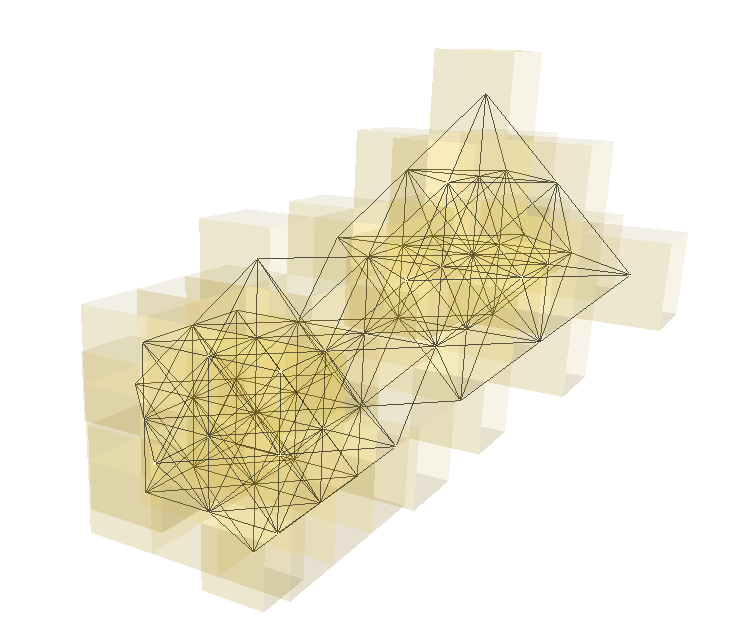
\includegraphics[width=0.4\textwidth]{object-3d-18-6} & 
        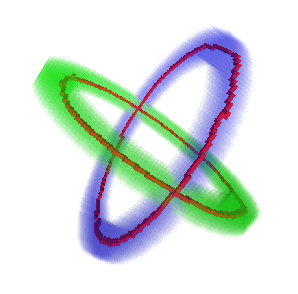
\includegraphics[width=0.3\textwidth]{thinning-3d} \\
        Adjacencies &
        thinning in (6,26) \\
      \end{tabular}
    }

    \only<2-3>{
    \item cubical cellular topology + algebraic topology
      \only<2>{
        \begin{itemize}
        \item cells, adjacent and incident cells, faces and cofaces
        \item signed cells, signed incidence, boundary operators
        \end{itemize}

        \begin{tabular}{cc}
          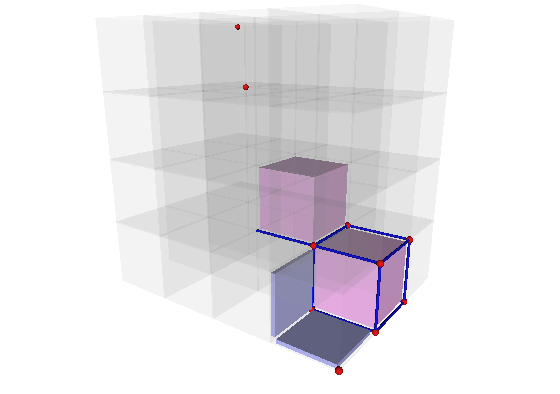
\includegraphics[width=0.4\textwidth]{3DKhalimskyCells}&
	  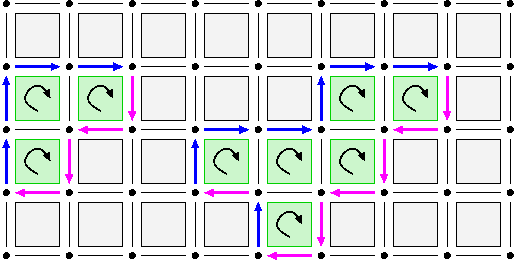
\includegraphics[width=0.4\textwidth]{Boundaries}\\
        \end{tabular}
      }
    }
    \only<3>{
    \item digital surface topology ({\em \`a la Herman})
      \begin{itemize}
      \item surfels, surfel adjacency, surfel neighborhood
      \item surface tracking (normal, fast), contour tracking in $n$D
      \end{itemize}

      \begin{tabular}{cc}
        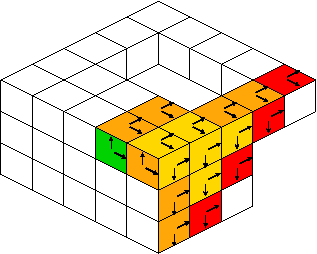
\includegraphics[width=0.4\textwidth]{suivi-artzy} &
        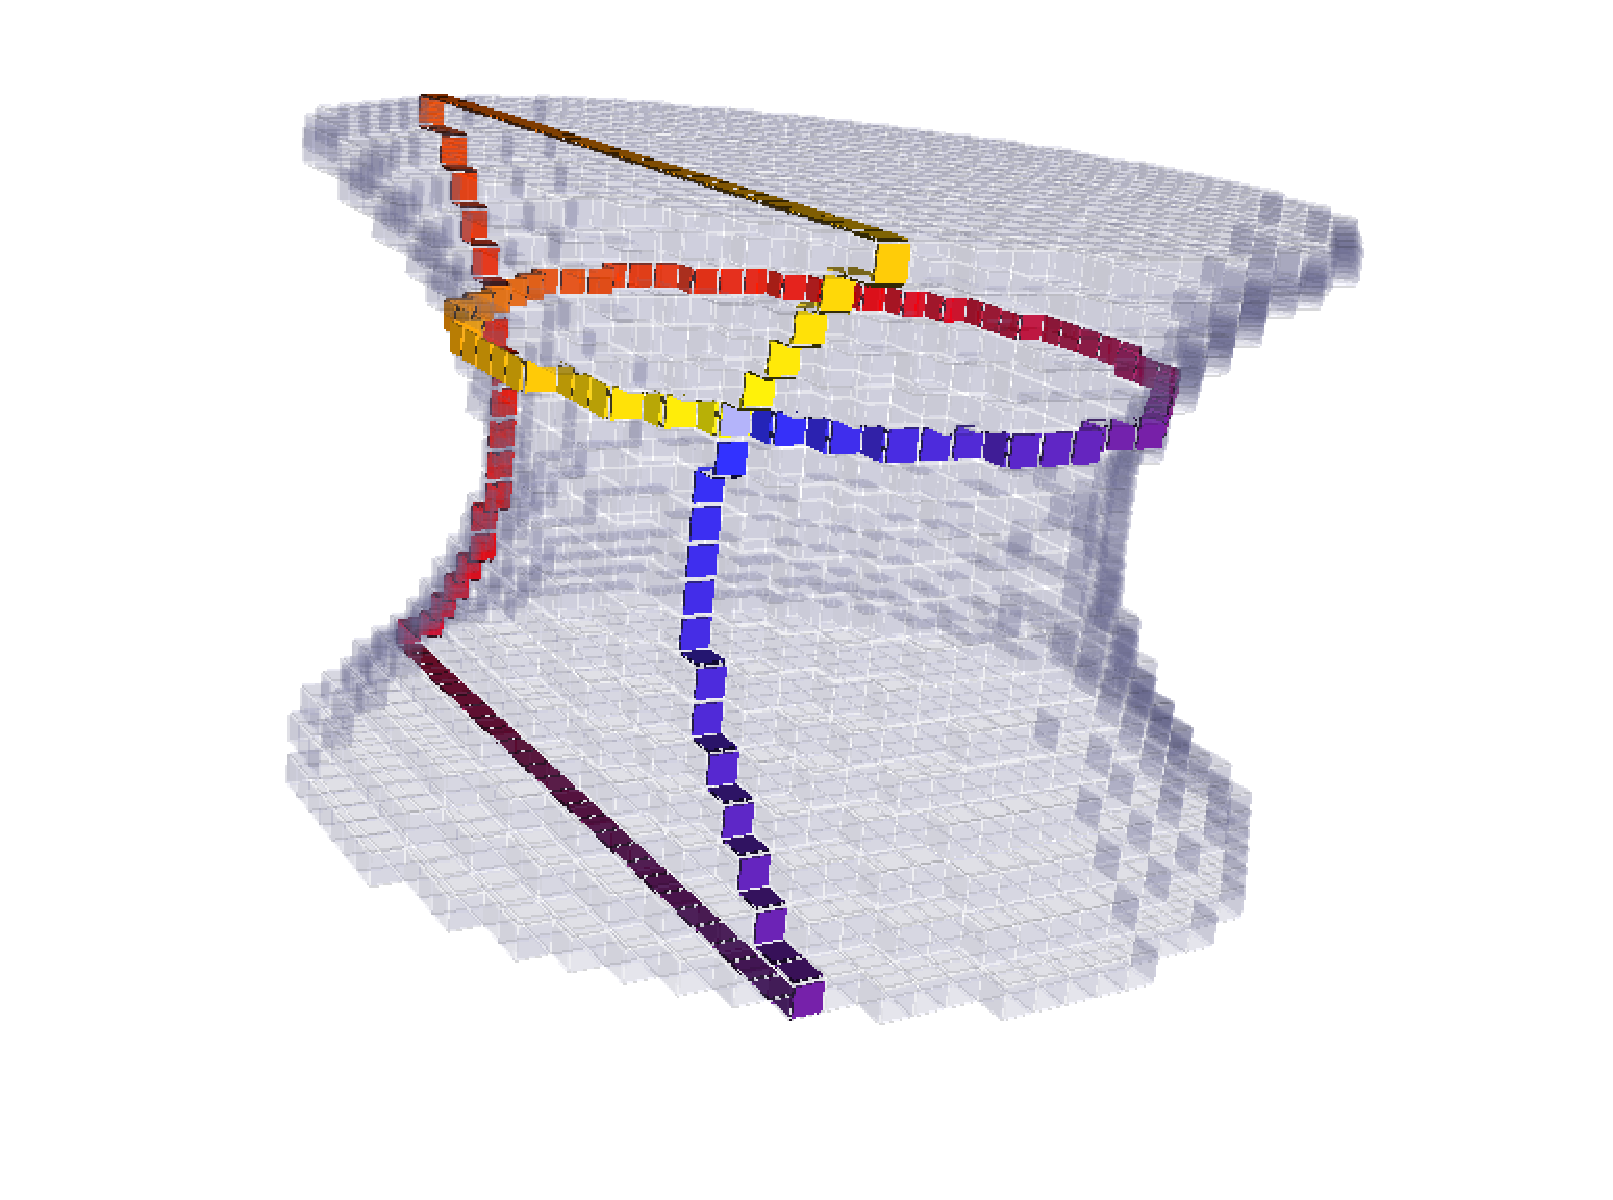
\includegraphics[width=0.4\textwidth]{surfelTracking} \\
      \end{tabular}
    }
  \end{enumerate}
\end{frame}
%------------------------------------------------------------------------------

%------------------------------------------------------------------------------
\begin{frame}%[allowframebreaks]
  \frametitle{Package Topology, \alertred{new} in DGtal 0.5}
  
  \begin{myblocklbluish}{\textwidth}{Digital Surface}
    $\begin{array}{c}
      \left.
      \begin{minipage}{0.5\textwidth}
        \begin{itemize}
        \item[] surfels / signed $n-1$-cells
        \item[$+$] adjacencies between surfels
        \end{itemize}
      \end{minipage}
      \right\}
      \begin{minipage}{0.45\textwidth}
        \begin{itemize}
        \item kind of "dual" graph
        \item kind of manifold
        \end{itemize}
      \end{minipage}
    \end{array}$
  \end{myblocklbluish}

  \only<1>{
    \mbox{~}\vspace{5mm}\\

    \begin{tabular}{ccc}
      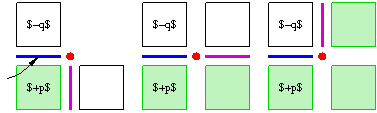
\includegraphics[height=1.5cm]{IntAdjacency}&
      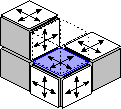
\includegraphics[height=1.5cm]{SurfaceTracking2}&
      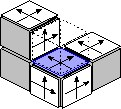
\includegraphics[height=1.5cm]{SurfaceTracking}\\
    \end{tabular}
  }

  \only<2>{
    \begin{enumerate}
    \item High-level {\tt DigitalSurface} class for representing any
      kind of digital surface
    \item Many container classes for digital surfaces
      \begin{itemize}
      \item boundary of digital shape
      \item boundary of implicitly defined shape
      \item set of surfels
      \item implicitly defined set of surfels
      \item light containers
      \end{itemize}
    \item a {\tt DigitalSurface} is a graph
    \item a {\tt DigitalSurface} is a combinatorial surface (with umbrellas)
    \end{enumerate}
  }

\end{frame}
%------------------------------------------------------------------------------

%------------------------------------------------------------------------------
\begin{frame}%[allowframebreaks]
  \frametitle{Direct applications}

  \begin{itemize}
    \item marching cubes algorithm
    \item tracking implicit polynomial surfaces
    \item representing boundary of regions and frontier between regions
    \item breadth-first visiting on surfaces
    \item estimating normals on surfaces
  \end{itemize}

  \begin{center}
  \begin{tabular}{ccccc}
    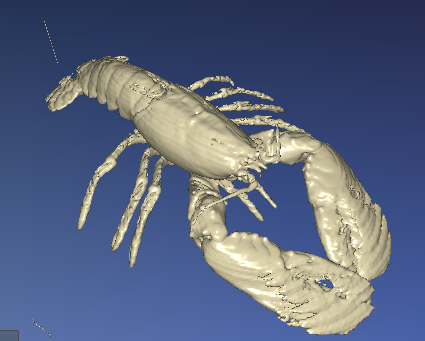
\includegraphics[width=0.18\textwidth]{mc-lobster-40}&
    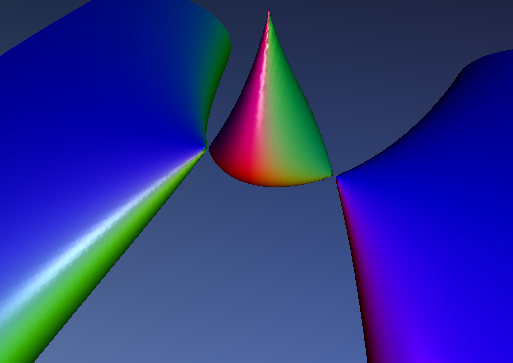
\includegraphics[width=0.18\textwidth]{polynomial-fun2}&
    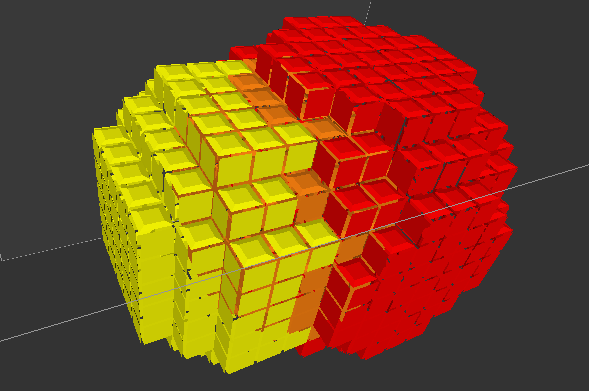
\includegraphics[width=0.18\textwidth]{digital-surface-intersecting-balls}&
    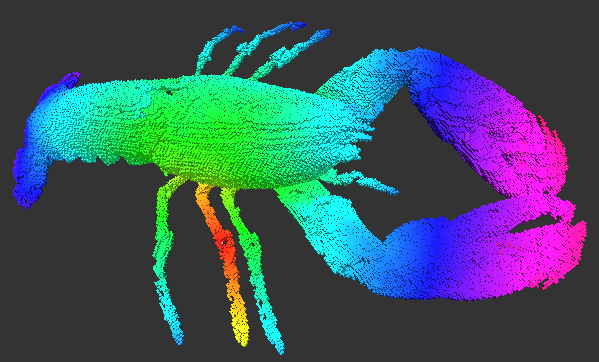
\includegraphics[width=0.18\textwidth]{digital-surface-bfv-lobster}&
    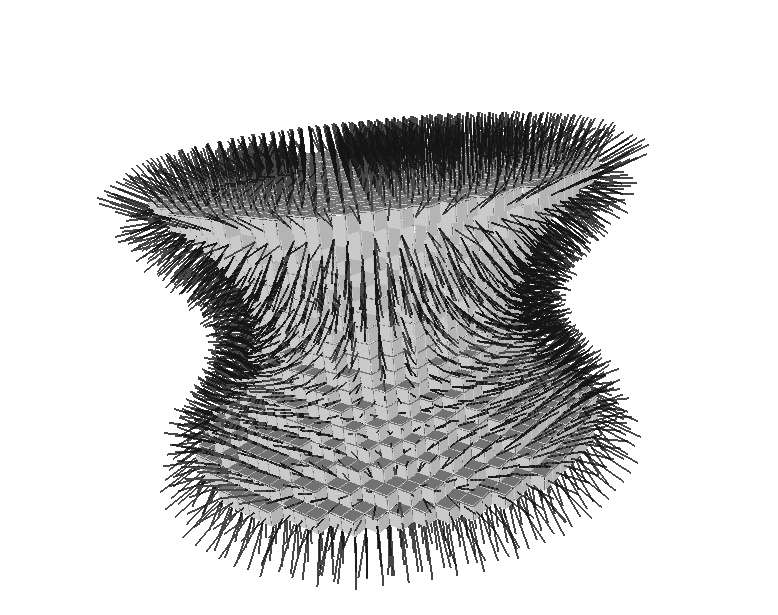
\includegraphics[width=0.18\textwidth]{normal-estimation}\\
  \end{tabular}
  \end{center}
\end{frame}
%------------------------------------------------------------------------------


%%%%%%%%%%%%%%%%%%%%%%%%%%%%%%%%%%%%%%%%%%%%%%%%%%%%%%%%%%%%%%%%%%%%%%%%%%%%%%%
\section{Principles and uses}
%%%%%%%%%%%%%%%%%%%%%%%%%%%%%%%%%%%%%%%%%%%%%%%%%%%%%%%%%%%%%%%%%%%%%%%%%%%%%%%

%------------------------------------------------------------------------------
\begin{frame}[fragile]%[allowframebreaks]
  \frametitle{Necessary concepts and classes for digital surfaces}

  \small 
  One must choose
  \begin{itemize}
  \item the representation of cellular grid space: model of
    \href{http://liris.cnrs.fr/dgtal/doc/nightly/structDGtal_1_1CCellularGridSpaceND.html}{\texttt{\alertred{CCellularGridSpaceND}}}\\
    e.g. \href{http://liris.cnrs.fr/dgtal/doc/nightly/classDGtal_1_1KhalimskySpaceND.html}{\texttt{\alert{KhalimskySpaceND}$<N,int>$}}, \texttt{\alert{Z2i::KSpace}}, \texttt{\alert{Z3i::KSpace}}

  \item the kind of adjacency between surfels, \href{http://liris.cnrs.fr/dgtal/doc/nightly/classDGtal_1_1SurfelAdjacency.html}{\texttt{\alert{SurfelAdjacency}$<N>$}}

  \item the kind of surface container: model of \href{http://liris.cnrs.fr/dgtal/doc/nightly/structDGtal_1_1CDigitalSurfaceContainer.html}{\texttt{\alertred{CDigitalSurfaceContainer}}}

  \end{itemize}
  
  \begin{lstlisting}
typedef Z3i::Point Point; // 3D digital point
typedef Z3i::Domain Domain; 
typedef Z3i::DigitalSet DigitalSet; // a set of digital points
typedef Z3i::KSpace KSpace; // 3D cellular grid space
typedef SurfelAdjacency<3> SAdj; // surfel adjacency.
typedef DigitalSetBoundary<KSpace,DigitalSet> Container; // kind of surface container
typedef DigitalSurface<Container> MyDigSurf; // concrete digital surface
  \end{lstlisting}
%% KSpace K; ...              // the cellular space
%% DigitalSet someShape(...); // the shape
%% SAdj surfAdj( true );      // the adjacency
%% Container surfContainer( K, someShape, surfAdj );
%% MyDigSurf digSurf( surfContainer );
%%   \end{lstlisting}

\end{frame}
%------------------------------------------------------------------------------

%------------------------------------------------------------------------------
\begin{frame}[fragile]%[allowframebreaks]
  \frametitle{Concrete instanciations for digital surfaces}

  Then, the chosen types are instantiated. Here \\
  digital surface = boundary of two intersecting balls
  \begin{lstlisting}
  Point p1( -20, -20, -20 ), p2( 20, 20, 20 );
  KSpace K; K.init( p1, p2, true ); // init space
  DigitalSet someShape( Domain( p1, p2 ) );
  Shapes<Domain>::addNorm2Ball( someShape, Point(-3,0,0), 4 );
  Shapes<Domain>::addNorm2Ball( someShape, Point(3,0,0), 4 );
  SAdj surfAdj( true );  // the adjacency
  Container surfContainer( K, someShape, surfAdj );
  MyDigSurf digSurf( surfContainer ); // digital surface
  \end{lstlisting}
  
  Using the digital surface (displays 518):
  \lstset{emph={size},emphstyle=\color{MyGreen}}
  \begin{lstlisting}
  cout << "- nb surfels/vertices = "
       << digSurf.size() << endl;
  \end{lstlisting}
  

\end{frame}
%------------------------------------------------------------------------------

%------------------------------------------------------------------------------
\begin{frame}[fragile]%[allowframebreaks]
  \frametitle{How to use digital surfaces (I)}

  Just enumerating its elements...
  \lstset{emph={begin,end,ConstIterator},emphstyle=\color{MyGreen}}
  \begin{lstlisting}
  QApplication application( argc, argv );
  Viewer3D viewer; // QGL viewer
  viewer.show(); 
  for( MyDigSurf::ConstIterator it = digSurf.begin(),
	   itend = digSurf.end(); it != itend; ++it )
    viewer << *it;
  viewer << Viewer3D::updateDisplay;
  return application.exec();
  \end{lstlisting}

  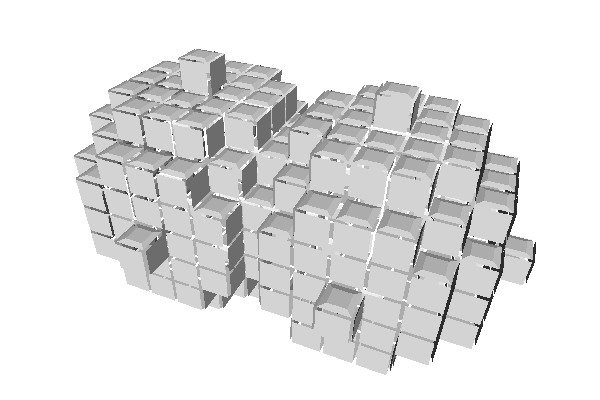
\includegraphics[width=0.5\textwidth]{two-balls}
\end{frame}
%------------------------------------------------------------------------------

%------------------------------------------------------------------------------
\begin{frame}[fragile]%[allowframebreaks]
  \frametitle{How to use digital surfaces (II)}

  Getting the neighbors and drawing the graph...
  \lstset{language=c++, numbers=left, tabsize=2, frame=single, breaklines=true, basicstyle=\ttfamily\tiny,
     numberstyle=\tiny\ttfamily, framexleftmargin=13mm, xleftmargin=12mm,keywordstyle=\color{blue}\bfseries,%
     commentstyle=\sffamily\color{red}}
  \lstset{emph={begin,end,ConstIterator,writeNeighbors},emphstyle=\color{MyGreen}}

  \begin{lstlisting}
  typedef std::vector<Vertex> Neighborhood;
  for ( ConstIterator it = digSurf.begin(),
          itend = digSurf.end(); it != itend; ++it )
    {
      Neighborhood N;
      back_insert_iterator<Neighborhood> itN = back_inserter( N );
      digSurf.writeNeighbors( itN , *it );
      Point p = K.sKCoords( *it );
      for ( unsigned int i = 0; i < N.size(); ++i )
        {
          Point q = K.sKCoords( N[ i ] );
          viewer.addLine ( p[0]/2.0, p[1]/2.0, p[2]/2.0,
                           q[0]/2.0, q[1]/2.0, q[2]/2.0, 
                           DGtal::Color ( 200,20,20 ), 2.0 );
        }
    }
  \end{lstlisting}
  \vspace{-0.6cm}
  \mbox{~}\hfill\fbox{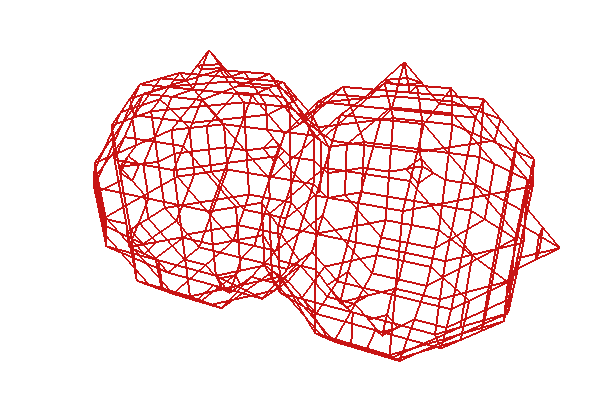
\includegraphics[width=0.4\textwidth]{two-balls-graph}}
%  \mbox{~}\hfill\parbox{0.45\textwidth}{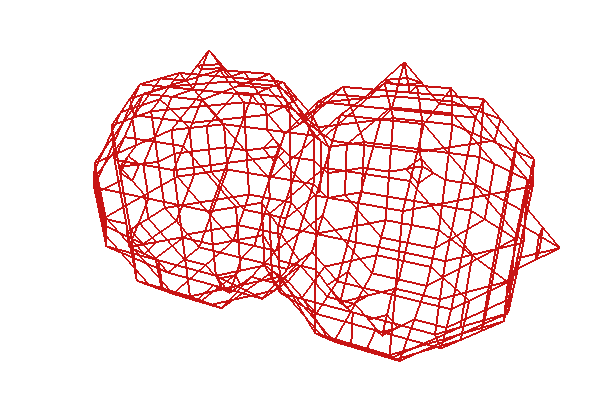
\includegraphics[width=0.45\textwidth]{two-balls-graph}}
\end{frame}
%------------------------------------------------------------------------------

%------------------------------------------------------------------------------
\begin{frame}[fragile]%[allowframebreaks]
  \frametitle{How to use digital surfaces (III)}

    \begin{myblocklbluish}{\textwidth}{Digital surfaces are combinatorial surfaces}
      \begin{columns}
        \begin{column}{0.65\textwidth}
          \only<1>{
            \begin{itemize}
            \item in $n$-D
            \item vertices = $n-1$-cells
            \item edges $\approx$ $n-2$-cells
            \item faces $\approx$ $n-3$-cells
            \end{itemize}
          }
          \only<2>{
            \begin{itemize}
            \item in \alertred{$3$-D}
            \item vertices = surfels
            \item edges $\approx$ linels
            \item faces = \alert{umbrellas}
            \end{itemize}
          }
        \end{column}
        \begin{column}{0.3\textwidth}
          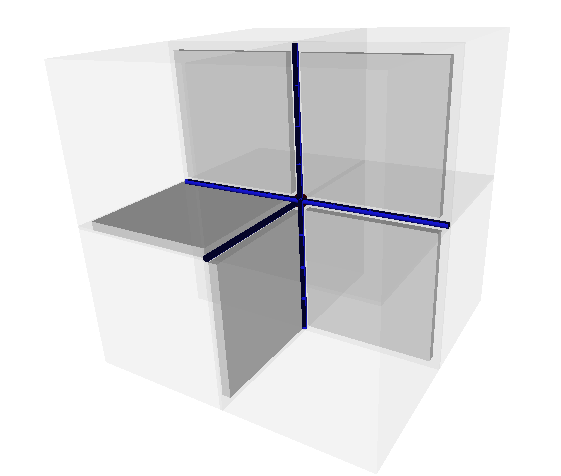
\includegraphics[width=0.95\textwidth]{umbrella}
        \end{column}
      \end{columns}
    \end{myblocklbluish}

    %\visible<2>{
      Inner types \alert{\tt Vertex, Arc, Face, xxxRange, xxxSet}
      \begin{lstlisting}
FaceRange   facesAroundVertex( const Vertex & v ) 
VertexRange verticesAroundFace( const Face & f )
FaceRange   facesAroundArc( const Arc & a )
FaceSet     allFaces()
FaceSet     allClosedFaces()
FaceSet     allOpenFaces() ...
      \end{lstlisting}
      %}
    
\end{frame}
%------------------------------------------------------------------------------

%------------------------------------------------------------------------------
\begin{frame}[fragile]%[allowframebreaks]
  \frametitle{How to use digital surfaces (IV)}

  Getting the faces and outputing their vertices

  \lstset{language=c++, numbers=left, tabsize=2, frame=single, breaklines=true, basicstyle=\ttfamily\tiny,
     numberstyle=\tiny\ttfamily, framexleftmargin=13mm, xleftmargin=12mm,keywordstyle=\color{blue}\bfseries,%
     commentstyle=\sffamily\color{red}}
  \lstset{emph={begin,end,FaceSet,VertexRange,allClosedFaces,verticesAroundFace},emphstyle=\color{MyGreen}}

  \begin{lstlisting}
  typedef typename FaceSet::const_iterator FaceSetIter;
  typedef typename VertexRange::const_iterator VertexRangeIter;
  FaceSet faces = digSurf.allClosedFaces();
  for ( FaceSetIter itf = faces.begin(), 
        itf_end = faces.end(); itf != itf_end; ++itf )
    {
      Face face = *itf;
      out << face.nbVertices;
      VertexRange vtcs = digSurf.verticesAroundFace( face );
      for ( VertexRangeIter itv = vtcs.begin(), 
            itv_end = vtcs.end(); itv != itv_end; ++itv )
        out << " " << index[ *itv ];
      out << std::endl;
    }
  \end{lstlisting}

  \begin{columns}
    \begin{column}{0.63\textwidth}
      e.g. export in OFF format
      \lstset{emph={exportSurfaceAs3DOFF,exportEmbeddedSurfaceAs3DOFF},emphstyle=\color{MyGreen}}
   \begin{lstlisting}
void exportSurfaceAs3DOFF ( std::ostream & out )

template <typename CellEmbedder>
void exportEmbeddedSurfaceAs3DOFF
( std::ostream & out, const CellEmbedder & cembedder ) 
   \end{lstlisting}
    \end{column}
    \begin{column}{0.3\textwidth}
      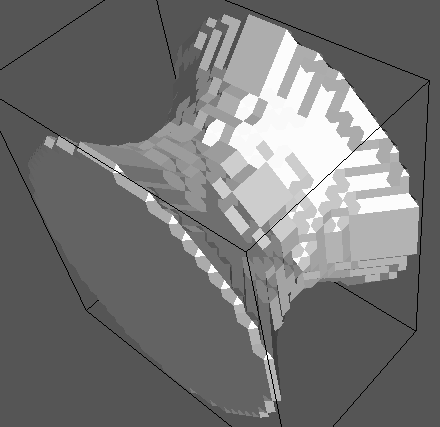
\includegraphics[width=\textwidth]{digital-surface-mc-cat10}
    \end{column}
  \end{columns}

\end{frame}
%------------------------------------------------------------------------------


%%%%%%%%%%%%%%%%%%%%%%%%%%%%%%%%%%%%%%%%%%%%%%%%%%%%%%%%%%%%%%%%%%%%%%%%%%%%%%%
\section{Containers}
%%%%%%%%%%%%%%%%%%%%%%%%%%%%%%%%%%%%%%%%%%%%%%%%%%%%%%%%%%%%%%%%%%%%%%%%%%%%%%%

%------------------------------------------------------------------------------
\begin{frame}%[allowframebreaks]
  \frametitle{Diversity of digital surfaces}

  \begin{itemize}
  \item may be open or closed
  \item may be connected or not
  \item may be defined explicitly with their surfels
  \item may be defined implicitly as the boundary of some shape
  \item the surfels may be listed or known only through a predicate
  \item the shape may be described by its points or known only through a predicate
  \item the surface may be big or infinite so that only lazy extraction is reasonnable
  \end{itemize}

  \small
  You wish to process them with the same object: {\tt \alert{DigitalSurface}$<$T$>$}

  $T$ is a model of \href{http://liris.cnrs.fr/dgtal/doc/nightly/structDGtal_1_1CDigitalSurfaceContainer.html}{\texttt{\alertred{CDigitalSurfaceContainer}}}
\end{frame}
%------------------------------------------------------------------------------

%------------------------------------------------------------------------------
\begin{frame}%[allowframebreaks]
  \frametitle{Partial architecture}

  \only<1>{
    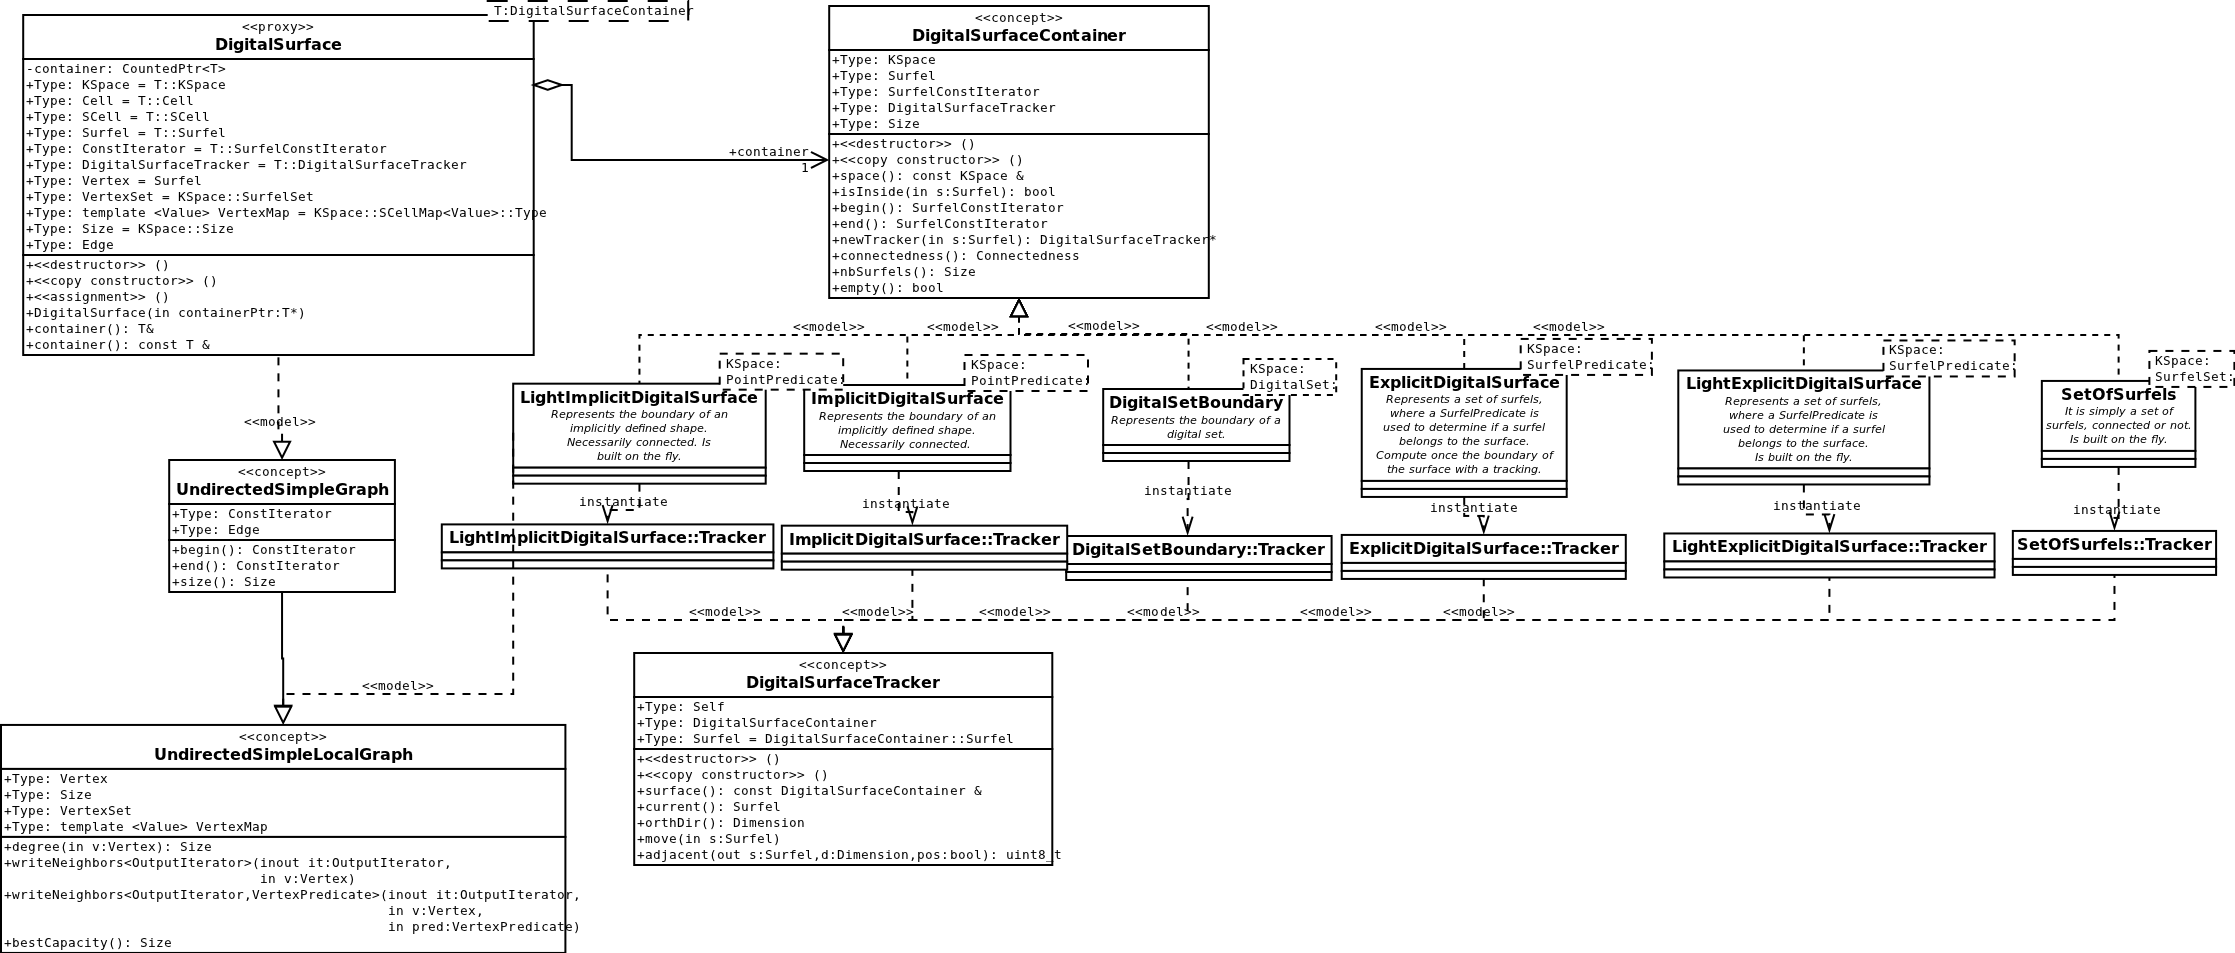
\includegraphics[width=\textwidth]{diag-digital-surface-1}
  }%
  \only<2>{
    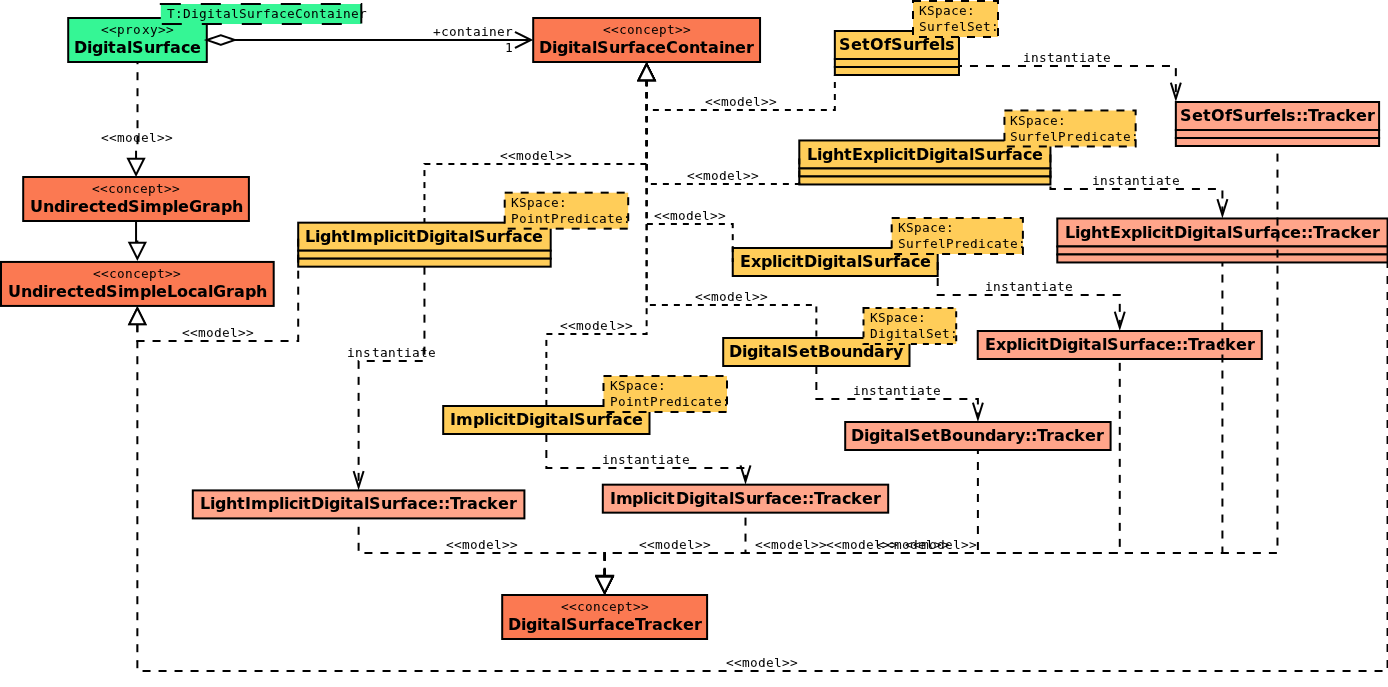
\includegraphics[width=\textwidth]{diag-digital-surface-1-simplified}
  }%
\end{frame}
%------------------------------------------------------------------------------

%------------------------------------------------------------------------------
\begin{frame}%[allowframebreaks]
  \frametitle{Digital surface containers}

\begin{itemize}[<+->]
\item \href{http://liris.cnrs.fr/dgtal/doc/nightly/classDGtal_1_1DigitalSetBoundary.html}{\texttt{\alert{DigitalSetBoundary}$<$KSpace,DigitalSet$>$}}
  Represents the boundary of a digital set (a set of
  digital points, considered as the set of pixels/voxels/spels of
  the space).

  \fbox{\small $\Rightarrow$ interpixel boundary of a digital shape}

\item \href{http://liris.cnrs.fr/dgtal/doc/nightly/classDGtal_1_1ImplicitDigitalSurface.html}{\texttt{\alert{ImplicitDigitalSurface}$<$KSpace,PointPredicate$>$}} Represents the (connected) boundary
  of shape defined implicitly by a predicate. $+$ \alert{\tt Light} version.
%%  Computes at instanciation the set of surfels by a tracking algorithm.

  \fbox{\small $\Rightarrow$ implicit surface computed once or on-the-fly}
  
\item \href{http://liris.cnrs.fr/dgtal/doc/nightly/classDGtal_1_1SetOfSurfels.html}{\texttt{\alert{SetOfSurfels}$<$KSpace,SurfelSet$>$}} Represents an arbitrary set of surfels stored
  explicitly.

  \fbox{\small $\Rightarrow$ arbitrary known surface: add topology to a set}

\item \href{http://liris.cnrs.fr/dgtal/doc/nightly/classDGtal_1_1ExplicitDigitalSurface.html}{\texttt{\alert{ExplicitDigitalSurface}$<$KSpace,SurfelPredicate$>$}} Represents a (connected) set of
  surfels defined implicitly by a predicate.  $+$ \alert{\tt Light} version.
%%  Computes at instanciation the set of surfels by a tracking algorithm.

  \fbox{\small $\Rightarrow$ frontier between regions in images, computed once or on-the-fly}

\end{itemize}
\end{frame}

%% - model ImplicitDigitalSurface, parameterized by a cellular space
%%   and a predicate Point->bool. Represents the (connected) boundary
%%   of shape defined implicitly by a predicate. Computes at
%%   instanciation the set of surfels by a tracking algorithm.
%% - model LightImplicitDigitalSurface, parameterized by a cellular
%%   space and a predicate Point->bool. Represents the (connected)
%%   boundary of shape defined implicitly by a predicate. Do not
%%   compute at instanciation the set of surfels, but rather visits
%%   the surface on demand.
%% - model SetOfSurfels, parameterized by a cellular space and a set
%%   storing surfels. Represents an arbitrary set of surfels stored
%%   explicitly.
%% - model ExplicitDigitalSurface, parameterized by a cellular space
%%   and a predicate Surfel->bool. Represents a (connected) set of
%%   surfels defined implicitly by a predicate. Computes at
%%   instanciation the set of surfels by a tracking algorithm.
%% - model LightExplicitDigitalSurface, parameterized by a cellular space
%%   and a predicate Surfel->bool. Represents a (connected) set of
%%   surfels defined implicitly by a predicate.  Do not
%%   compute at instanciation the set of surfels, but rather visits
%%   the surface on demand.

%------------------------------------------------------------------------------
\begin{frame}[squeeze]%[allowframebreaks]
  \frametitle{Package description}

  \begin{myblocklbluish}{\textwidth}{Should contain}
    \begin{itemize}
      \small
    \item classical digital topology {\em à la} Rosenfeld
    \item cartesian cellular topology
    \item digital surface topology {\em à la} Herman
    \item must be the base block of geometric algorithms
    \end{itemize}
  \end{myblocklbluish}
  \begin{myblocklgreenish}{\textwidth}{Examples}
    \begin{itemize}
      \small
    \item adjacencies, connected components, simple points, thinning
    \item cells, boundary operators, incidence, opening, closing
    \item contours, surfel adjacency, surface tracking
    \item topological invariants
    \end{itemize}
  \end{myblocklgreenish}
  \begin{myblocklredish}{\textwidth}{Location}
    \begin{itemize}
      \small
    \item \texttt{\{DGtal\}/src/DGtal/topology}
    \item \texttt{\{DGtal\}/src/DGtal/helpers}
    \item \texttt{\{DGtal\}/tests/topology}
    \end{itemize}
  \end{myblocklredish}

\end{frame}
%------------------------------------------------------------------------------


\end{document}
